\documentclass[12pt]{article}

\usepackage{tikz}
\usetikzlibrary{backgrounds}
\usepackage{graphicx}
\usepackage{amsmath}
\usepackage{amsthm}
\usepackage{amssymb}
\usepackage{url}
\usepackage{multirow}
\usepackage{times}
\usepackage{fullpage}
\usepackage{wrapfig}
\newcommand{\comment}[1]{}

\title{CS685: Group 14 \\
Distributed Code Revision Control System}
\author{
\begin{tabular}{ccc}
Satvik Chauhan & Rahul Ajmera \\
\url{satvikc@iitk.ac.in} & \url{rahulaaj@iitk.ac.in} \\
Dept. of CSE & Dept. of CSE \\
\multicolumn{2}{c}{Indian Institute of Technology, Kanpur}
\end{tabular}
}
\date{	% replace by ``initial'' or ``final'' as appropriate
\today}	% replace by actual date of submission or \today

\begin{document}
\maketitle
\begin{abstract}
A distributed revision control system (DRCS), distributed version control or
decentralized version control system (DVCS) keeps track of software revisions
and allows many developers to work on a given project without necessarily
being connected to a common network \cite{wiki}. Some of the popular
distributed version control systems are Git \cite{git}, Mercurial
\cite{mercurial}, darc \cite{darcs}, GNU Bazaar \cite{bazaar} etc. Distributed Version Control
Systems usually follow peer to peer approach rather than client server. So
instead of a central repository to which each client can synchronize their
changes, each peer has a working copy of the codebase. DVCS usually perform
syncronizations by exchanging patches between peers.

In this project we will be implementing a distributed version control
system with basic features like commit, push patch, pull patch, view history,
merging of code files, reverting changes etc.
\end{abstract}
\section{Introduction}
Talk about use of revision control systems.
asd
sayas
d
sa
ds
ad
as
d
as
d
as

add

asda

addsd
a
add

\begin{wrapfigure}[14]{r}{9cm}
\centering
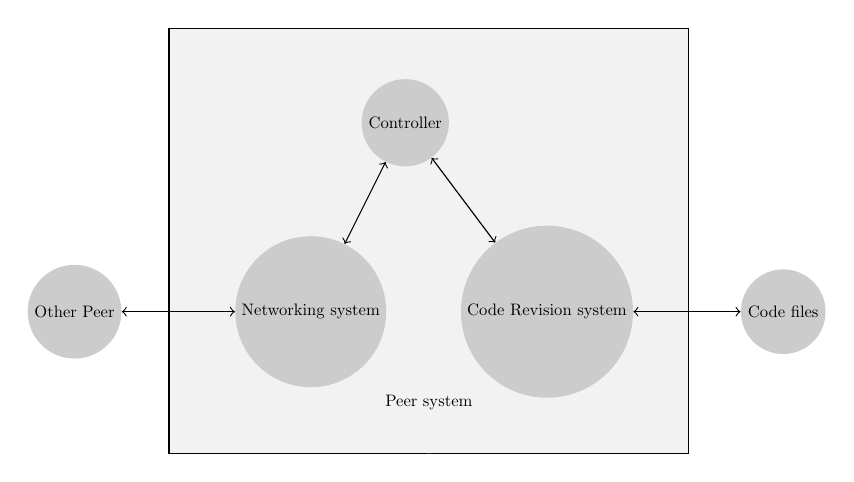
\begin{tikzpicture}[ scale=0.6,transform shape]
\tikzstyle{every node}=[circle,fill=gray!40]
\draw [fill=gray!10] (-3,-3) rectangle (8,6);
\draw (2.5,-3) node [above ,fill=gray!10] {Peer system};
\node (a) at (0,0) {Networking system} ;
\node (b) at (5,0) {Code Revision system};
\node (c) at (2,4) {Controller};
\node (f) at (10,0) {Code files};
\node (u) at (-5,0) {Other Peer};
\draw [<->] (c) -- (a);
\draw [<->] (c) -- (b);
\draw [<->] (u) -- (a);
\draw [<->] (b) -- (f);
\end{tikzpicture}
\caption{Highlevel design}
\end{wrapfigure}
\section{Implementation}
We take a peer to peer approach for maintaining the code. Every peer will have
its own copy of the codebase and can request other peers to merge their code
with his own codecopy. Unlike CVS, we do not keep a central repository and
every copy of the codebase is a valid working copy. The syncronization between
peers is be done by sending the commits which are not available at host. The
files common between commits are just treated as one file. We use
\emph{Deflate} text compression algorithm to compress the text files to
optimize network bandwith.

There are two ways of keeping the history of files at the time of
commits. One approach was to keep the base file and the incremental changes
after each commit. Although such approach seems optimal for storage
consumptions but is overly complicated and also a corruption of one file might
corrupt all your further commits. There are version controls that follow this
kind of history storage like Darcs \cite{darcs}. At the time of rollback you
need to make all the commits by applying incremental patches. Thus the
algorithm is not very optimal for rollbacks.

The storage nowdays is very cheap and the code files take very less amount of
storage space. So we can have the tradeoff of storage versus the complexity of
the algorithm.  Folowing the KISS \cite{KISS} principle, a very simple
algorithm could be to store snapshots. At the time of commit a snapshot of the
current working directory is taken. So after each commit the snapshot is added
to the list of existing snapshots.  The space consumption of such an algorithm
is proportional to number of commits which seems to be huge. But keeping
snapshots for each commit allows easy rollback, as you have the whole
directory with you at time of snapshot so you just copy those files to the
current working directory. With a basic assumption we can really optimize the
space consumption of our algorithm. The assumtion is that between commits
there are very few files which are actually modified. So we store files in a
single object directory with the names that correspond to the hash of its
content and keeping track of this mapping commit wise. Thus the files which
are unchanged between commits will have the same content and thus the same
name and will be saved as a single file rather than two different files as was
the case previously. To be more agressive we can further compress the text
files . This is very similar to the git's approach of compressing the
snapshots into blobs \cite{parable}.

\subsection{Networking}
Networking subsystem implements the underlying communication between the
peers. It consists of
\begin{itemize}
\item Defining the underlying protocol for communication.
\item Connecting to a peer and transferring the patches reported by the
  revision system.
\end{itemize}
We have used the python twisted library to implement our networking
system. Twisted's spread module provides framework to quickly and easily
implement peer to peer systems. Spread is a kind of RPC (Remote procedural
Calls) which allows us to make remote function calls. The parameters of the
functions as well as the returned element must have serializable instances. It
also allows to pass objects (which inherit from Copyable class) as parameters
to function calls.

The programming style for implementing spread application is asynchronous. It
adds callback to all the remote calls. The call methods are invocated when the
remote procedure returns the result. Thus it ensures that the execution at the
client side continues while the execution of the remote procedure is taking
place. We can also add the error callback which is invocated when an error is
raised at the server side. Thus the remote calls add some bit of transparency
avoiding any overhead due to network latency by being asynchronous.

\subsection{Code Revision System}
\begin{wrapfigure}[8]{r}{9cm}
\centering
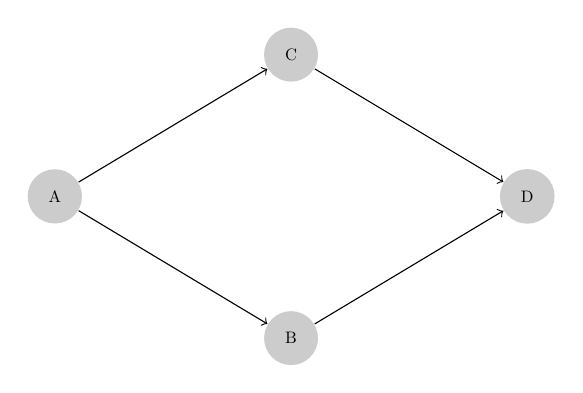
\begin{tikzpicture}[ scale=0.6,transform shape]
\tikzstyle{every node}=[circle,thick,fill=gray!40,inner sep=8]
\node (a) at (0,0) {A} ;
\node (b) at (5,-3) {B};
\node (c) at (5,3) {C};
\node (d) at (10,0) {D};
\draw [->] (a) -- (b);
\draw [->] (a) -- (c);
\draw [->] (b) -- (d);
\draw [->] (c) -- (d);
\end{tikzpicture}
\caption{3-way Merge Strategy}
\end{wrapfigure}
Code Revision system performs all the major tasks of creating blobs, patches and
keeping track of various versions of the code. It consists of
\begin{itemize}
\item Creating blobs and patches based on changes in the files.
\item Determining what patches needs to be send to the peer depending on the
  code version.
\item Merging of the patches to the codebase.
\end{itemize}
\subsection{User Interface/Controller}
This will provide the actual interface which user will be able to use and this
will coordinate the working of the other two components.
It consists of
\begin{itemize}
\item Defining a command line interface for linux machines and if possible a
  gui interface may be considered.
\item Defining the ususal commands like commit, push changes, pull changes
  etc.
\item This will act like a bridge between the networking subsystem and code
  revision system and will combine the features of both to provide an end to
  end distributed version control system.
\end{itemize}

\begin{thebibliography}{99}
\bibitem{wiki}
wikipedia \url{http://en.wikipedia.org/wiki/Distributed_revision_control}
\bibitem{git}
git version control system \url{http://git-scm.com}
\bibitem{mercurial}
Matt Mackall, \emph{Towards a Better SCM: Revlog and Mercurial} .
\bibitem{darcs}
Judah Jacobson, \emph{A formalization of Darcs patch theory using inverse
  semigroups}.
\bibitem{bazaar}
GNU Bazaar, \url{http://wiki.bazaar.canonical.com/}
\bibitem{parable}
Git Parable,
\url{http://tom.preston-werner.com/2009/05/19/the-git-parable.html}
\bibitem{KISS}
Keep it Simple, Stupid
\url{http://people.apache.org/~fhanik/kiss.html}
\end{thebibliography}

\end{document}